\begin{center}
	\LARGE
	Uden hjælpemidler
\end{center}

\begin{opgavetekst}{Opgave 1}
	En funktion $f$ er givet ved
	\begin{align*}
		f(x) = -\frac{1}{2}x^2 + \frac{5}{2}x - 2.
	\end{align*}
	Grafen for $f$ samt et markeret område $M$ kan ses på Figur \ref{fig:opg1}
	\begin{figure}[H]
		\centering
		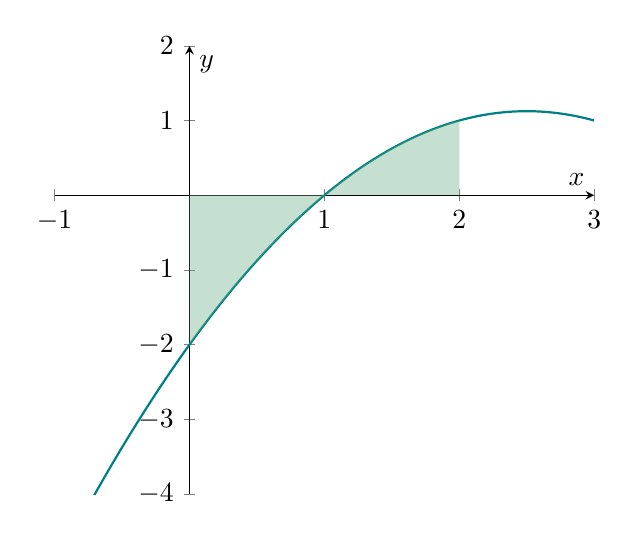
\begin{tikzpicture}
		\begin{axis}[
			axis lines = center, 
			xmin = -1, xmax = 3,
			ymin = -4, ymax = 2,
			xtick = {-3,-2,...,3,4},
			ytick = {-4,-3,...,3,4},
			xlabel = $x$, ylabel = $y$,
		]
			\addplot[color = teal, domain = -2:4, thick, samples = 500] {-0.5*x^2 + 2.5*x - 2};
			\fill[color = SeaGreen!70, opacity = 0.4 ]
			(axis cs: 0,0) -- 
			plot[domain = 0:2, variable = \x] (axis cs: \x, {-0.5*(\x)^2+2.5*\x - 2}) --
			(axis cs: 2,0) -- cycle;
		\end{axis}
		\end{tikzpicture}
		\caption{Markeret areal.}
		\label{fig:opg1}
	\end{figure}
	\phantom{h}
\end{opgavetekst}
\begin{delopgave}{1}
	Bestem arealet af området $M$.
\end{delopgave}

\begin{opgavetekst}{Opgave 2}
	En funktion $g$ er givet ved
	\begin{align*}
		g(x) = 3x^2 - 4x + c.
	\end{align*}
\end{opgavetekst}
\begin{delopgave}{1}
	Udnyt, at $g(-2) = 10$ for at bestemme tallet $c$.  
\end{delopgave}
\begin{delopgave}{2}
	Bestem den stamfunktion til $g$, der går gennem punktet $(2,1)$.
\end{delopgave}

\newpage

\begin{opgavetekst}{Opgave 3}
	Funktionen $h$ er givet ved
	\begin{align*}
		h(t) = \frac{t^3}{\sqrt{t^4+1}}
	\end{align*}
\end{opgavetekst}
\begin{delopgave}{1}
	Bestem $\int h(t) dt$.
\end{delopgave}

\begin{opgavetekst}{Opgave 4}
\end{opgavetekst}
\begin{delopgave}{1}
	Bestem integralet
	\begin{align*}
		\int_1^{e^{x^2}} \frac{1}{2x\sqrt{\ln(x)}} dx
	\end{align*}
\end{delopgave}

\newpage

\begin{center}
	\LARGE
	Med hjælpemidler
\end{center}



\begin{opgavetekst}{Opgave 5}
	\begin{center}
	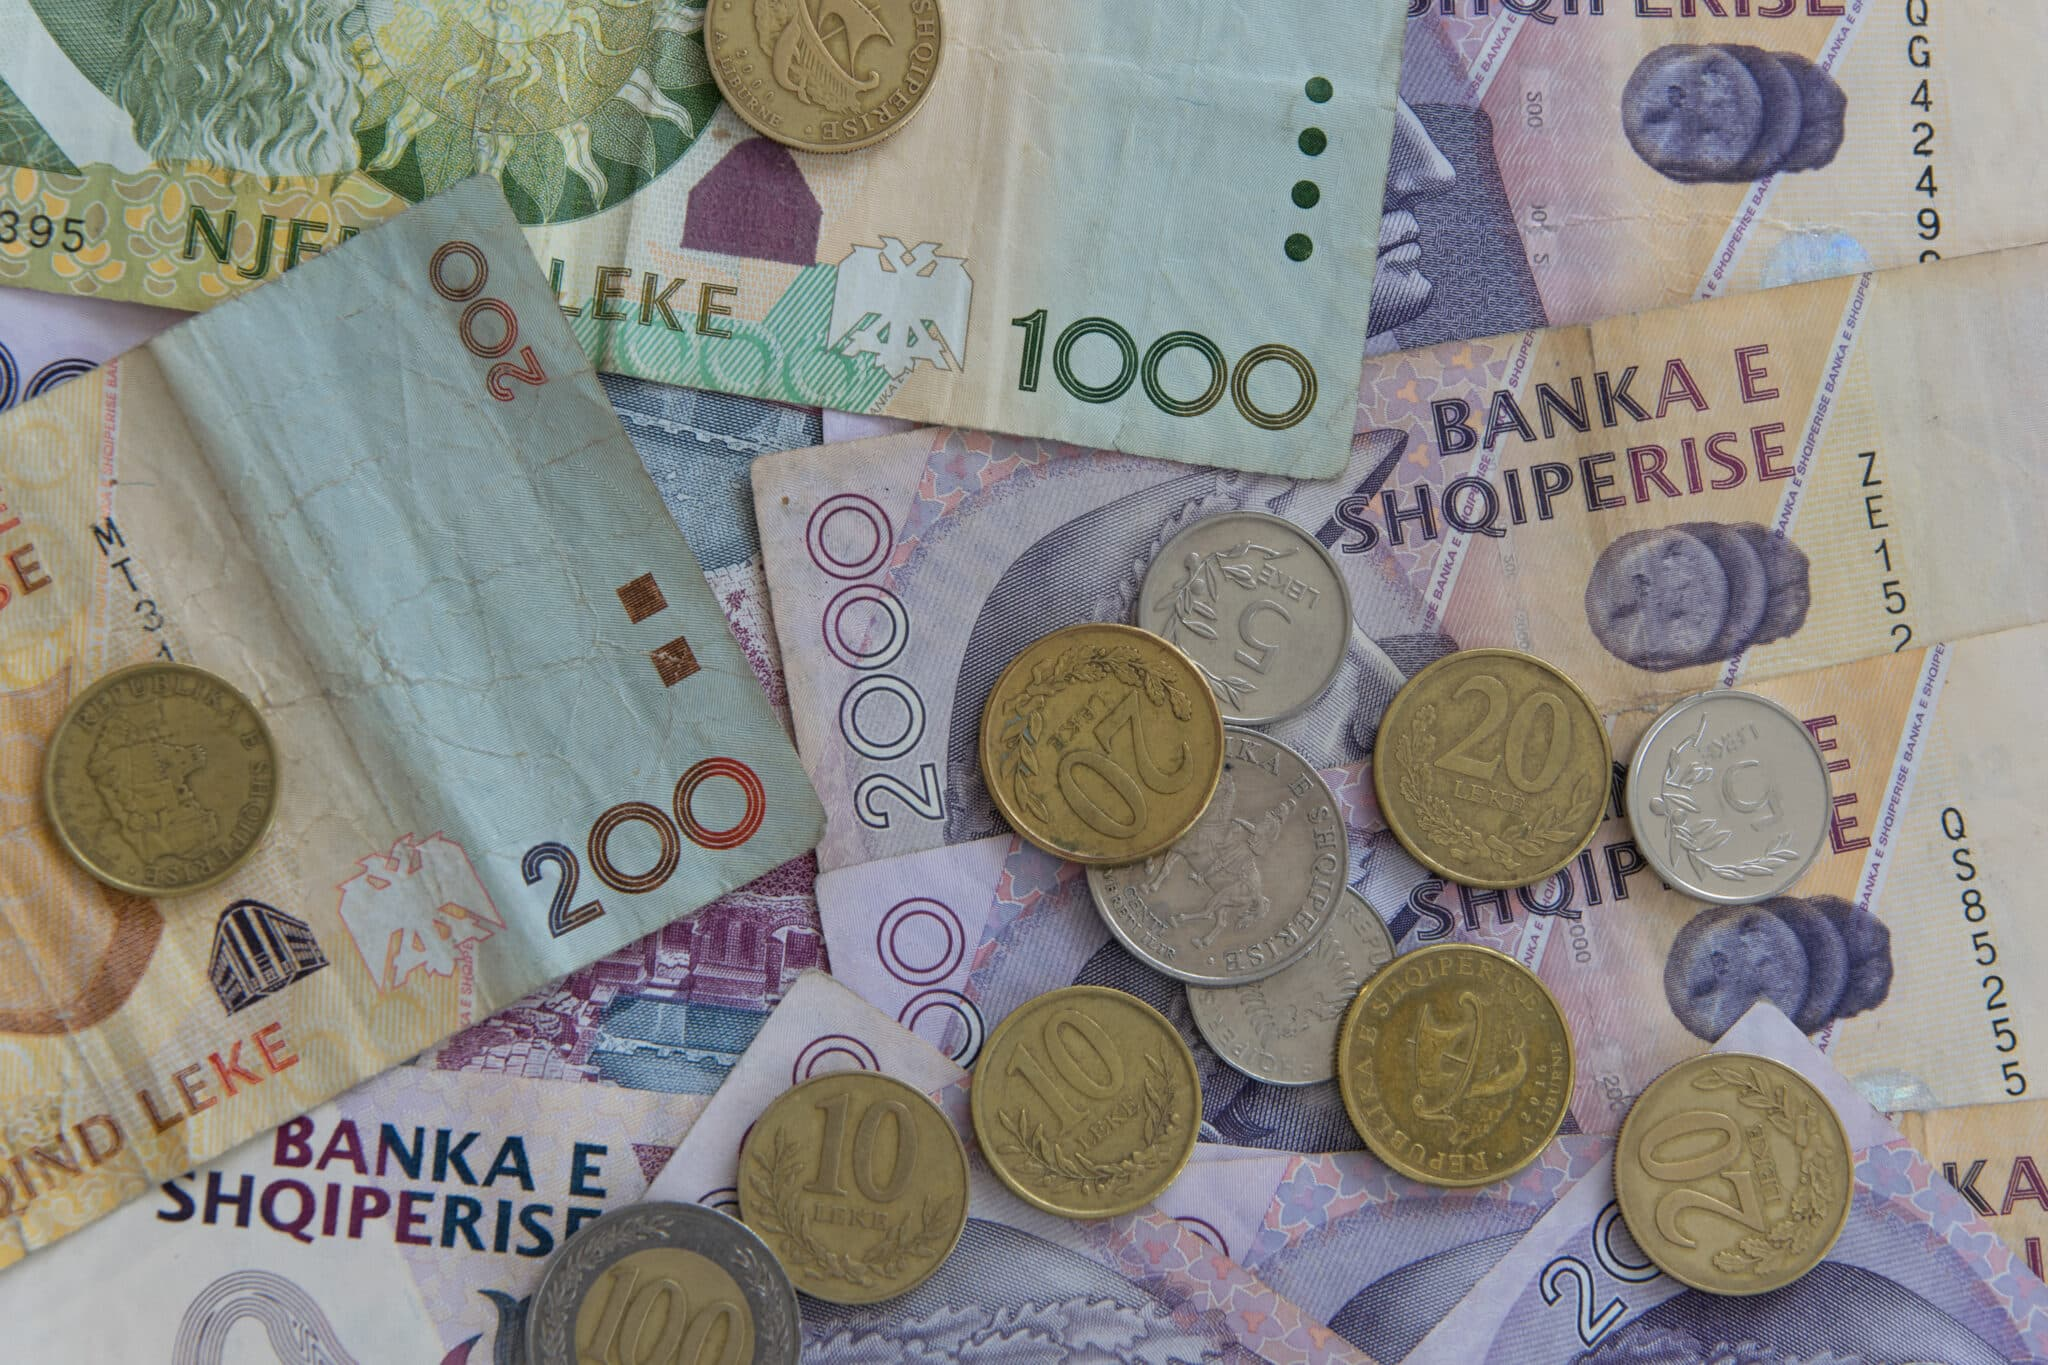
\includegraphics[width=0.5\textwidth]{Billeder/lek}
	\end{center}
	Prisen på den albanske møntfod lek (ALL) i kroner (DKK) siden 2015 kan findes i 
	\href{https://github.com/ChristianJLex/TeachingNotes/raw/master/2025-2026/Data%20og%20lign/LekKurs.xlsx}{\color{blue!60}dette datasæt.} 
	Det antages, at sammenhængen mellem prisen i DKK og antallet af måneder siden januar 2015 i perioden er givet ved
	\begin{align*}
		p(x) = ax^2 + bx + c.
	\end{align*}
\end{opgavetekst}
\begin{delopgave}{1}
	Anvend regression til at bestemme tallene $a$, $b$ og $c$. 
\end{delopgave}
\begin{delopgave}{2}
	Bestem tidspunktet, hvor prisen ifølge modellen vil overstige 0.1 krone per lek.
\end{delopgave}
\begin{delopgave}{3}
	Anvend integralregning til at bestemme den gennemsnitlige pris på lek fra januar 2015 til januar 2025.
\end{delopgave}

\begin{opgavetekst}{Opgave 6}
	Funktionen $f$ givet ved
	\begin{align*}
		f(x) = 3(x^2+1)^{0.5} -2.5
	\end{align*}
	udgør på intervallet $[-2,2]$ overfladen af en yo-yo. Yo-yoen dannes, når $f$ roteres omkring $x$-aksen. Alle 
	enheder er i cm. 
\end{opgavetekst}
\begin{delopgave}{1}
	Tegn grafen for $f$ for punkterne $(x,y) \in [-2,2]\times [-3,3]$
\end{delopgave}
\begin{delopgave}{2}
	Bestem rumfanget af yoyoen. 
\end{delopgave}

                 
\begin{opgavetekst}{Opgave 7}
	\begin{center}
		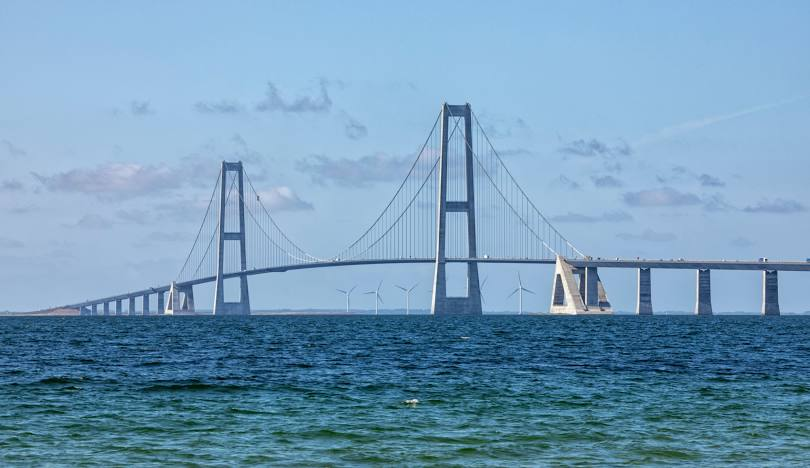
\includegraphics[width = 0.5\textwidth]{Billeder/storebelt}
	\end{center}
	Kablet mellem pylonerne på storebeltsbroen kan beskrives ved polynomiet $p$ givet ved
	\begin{align*}
		p(x) = 0.00027907x^2 - 0.4532x + 254, \ 0 \leq x \leq 1624, 
	\end{align*}
	hvor $x$ er afstanden fra den vestlige pylon og $p$ er højden af kablet. Alle enheder er i meter.
\end{opgavetekst}
\begin{delopgave}{1}
	Bestem højden af pylonerne. 
\end{delopgave}
\begin{delopgave}{2}
	Bestem længden af kablet mellem pylonerne. 
\end{delopgave}

\begin{opgavetekst}{Opgave 8}
	\begin{center}
		
\includegraphics[width= 0.5\textwidth]{Billeder/f1}
	\end{center}
	En Formel-1-bil kan accelerere fra $0\frac{m}{s}$ til $56\frac{m}{s}$ på ca. 3.9 sekunder.  
\end{opgavetekst}
\begin{delopgave}{1}
	Hvis accelerationen er konstant, hvad er så accelerationen for bilen henover de første 3.9 sekunder?
\end{delopgave}
\begin{delopgave}{2}
	Hvor langt har bilen kørt efter 3.9 sekunder?
\end{delopgave}
\begin{meretekst}
	Bilen kan bremse med en acceleration på ca. $-5g$ eller $-49.1\frac{m}{s^2}$. 
\end{meretekst}
\begin{delopgave}{3}
	Afgør, hvor langt bilen skal bruge for at bremse ned fra $56\frac{m}{s}$ igen, hvis bilen kan bremse med en konstant 
	acceleration.
\end{delopgave}